
\documentclass[a4paper, 12pt]{article}

\usepackage{amsmath}
\usepackage{amssymb}
\usepackage{graphicx}
\usepackage{listings}[language=Python]
\lstdefinestyle{mystyle}{
    breakatwhitespace=false,         
    breaklines=true,                 
    captionpos=b,                    
    keepspaces=true,                 
    numbers=left,                    
    numbersep=5pt,                  
    showspaces=false,                
    showstringspaces=false,
    showtabs=false,                  
    tabsize=2
}

\lstset{style=mystyle}

\title{Lab-05 Report}
\author{st122246}

\begin{document}
	\maketitle

	\section{Q1: ORB/AKAZE Tutorial}

	\begin{figure}
		\caption{Q1: ORB/AKAZE Tutorial}
		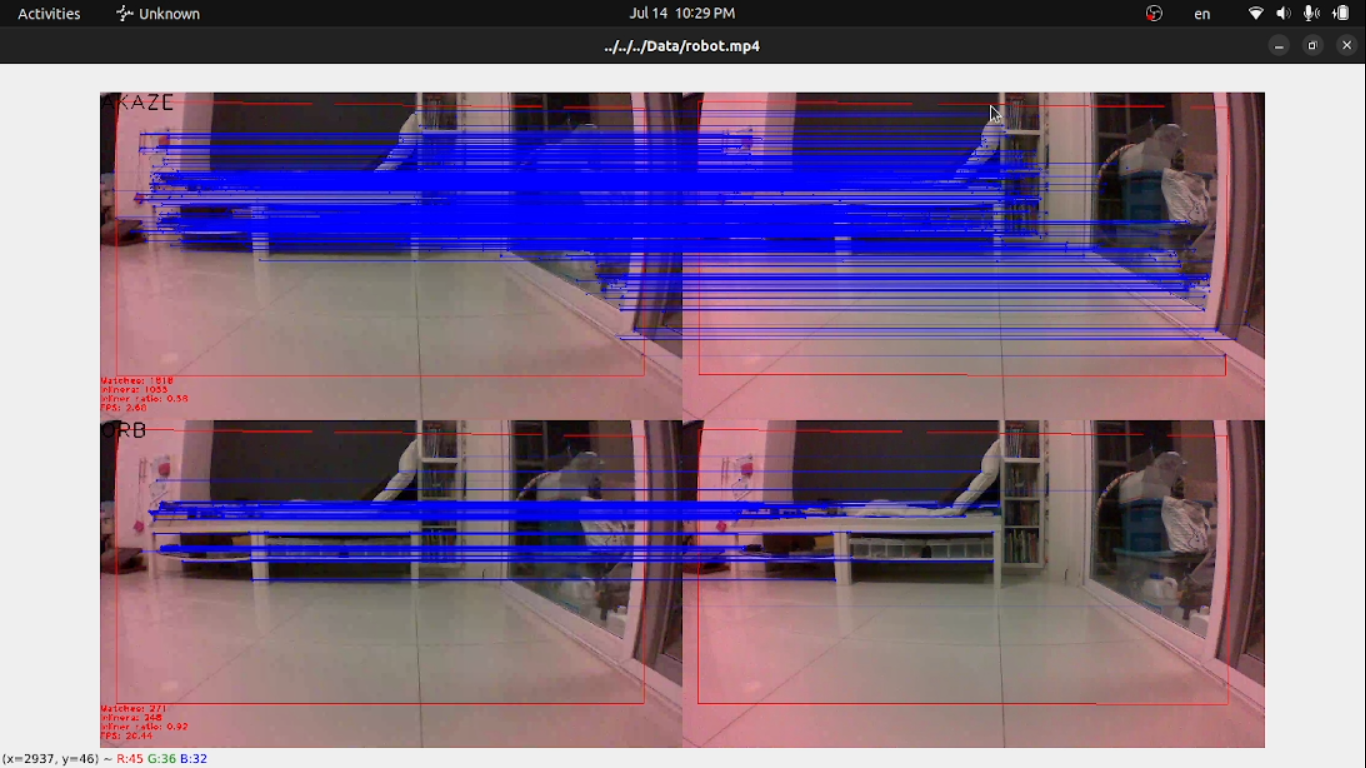
\includegraphics[scale=0.25]{img/akaze_orb.png}
	\end{figure}

	\section{Q2:  Feature Points}	
	
    Detect feature points
    \begin{lstlisting}
# ----------- Create detector -----------
detector1 = cv.AKAZE_create()
detector2 = cv.ORB_create()

def detect_key_points(self):
    """
    Detect features in two frames.
    """
    img1_kps, img1_desc = self.detector.detectAndCompute(self.img1, None)
    img2_kps, img2_desc = self.detector.detectAndCompute(self.img2, None)

    res_img1 = cv.drawKeypoints(self.img1, img1_kps, None, (255, 0, 0), cv.DRAW_MATCHES_FLAGS_DRAW_RICH_KEYPOINTS)
    res_img2 = cv.drawKeypoints(self.img2, img1_kps, None, (255, 0, 0), cv.DRAW_MATCHES_FLAGS_DRAW_RICH_KEYPOINTS)

    res_img1 = cv.putText(res_img1, "Image 1", (0, 60), cv.FONT_HERSHEY_PLAIN, 3, (0, 0, 255), 2)
    res_img2 = cv.putText(res_img2, "Image 2", (0, 60), cv.FONT_HERSHEY_PLAIN, 3, (0, 0, 255), 2)

    res_img = cv.hconcat([res_img1, res_img2])

    self._img1_kps = img1_kps
    self._img1_desc = img1_desc
    self._img2_kps = img2_kps
    self._img2_desc = img2_desc

    return res_img, img1_kps, img1_desc, img2_kps, img2_desc
    \end{lstlisting}

    \begin{figure}
		\caption{Q2: Feature Points}
		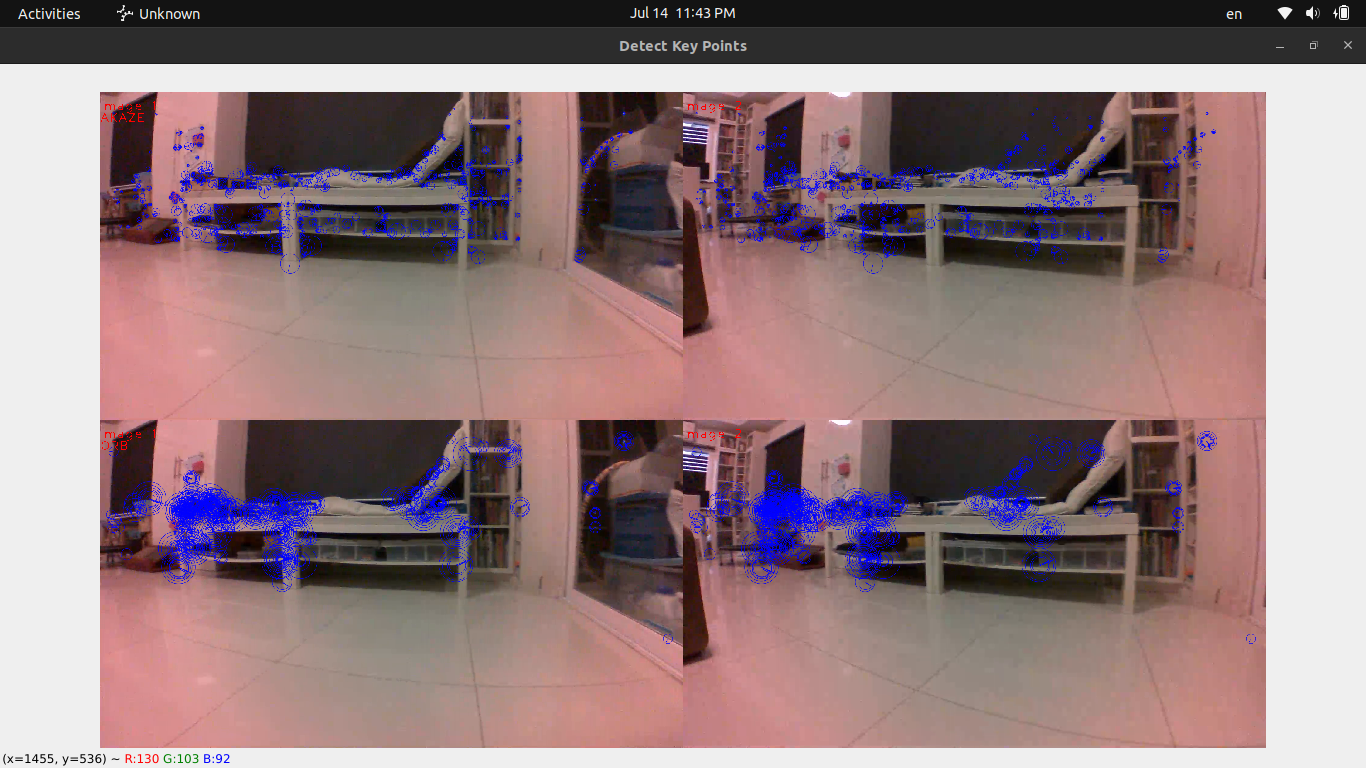
\includegraphics[scale=0.25]{img/feature_points.png}
	\end{figure}

    \section{Q3: Undistortion}

    \begin{lstlisting}
def _undistorted_image(self, image):
    h, w = image.shape[:2]
    new_camera_mtx, roi = cv.getOptimalNewCameraMatrix(self.camera_mtx, self.camera_dist, (w, h), 1, (w, h))
    undistorted_img = cv.undistort(image, self.camera_mtx, self.camera_dist, None, new_camera_mtx)
    x, y, w, h = roi
    undistorted_img = undistorted_img[y:y+h, x:x+w]
    return undistorted_img, new_camera_mtx, x, y

def _undistorted_points(self, points, new_camera_matrix, new_x, new_y):
    undistorted_pts = cv.undistortPoints(points, self.camera_mtx, self.camera_dist, P=new_camera_matrix)
    undistorted_pts = np.array([[pt[0, 0]-new_x, pt[0, 1]-new_y] for pt in undistorted_pts], dtype=np.float32)
    return undistorted_pts

def _undistorted_key_points(self, key_points, new_camera_matrix, new_x, new_y):
    new_key_points = list()

    pts = np.array([keypoint.pt for keypoint in key_points], dtype=np.float32)
    undistorted_pts = self._undistorted_points(pts, new_camera_matrix, new_x, new_y)

    for i, (kp, pt) in enumerate(zip(key_points, undistorted_pts)):
        new_key_point = cv.KeyPoint(x=pt[0], y=pt[1], size=kp.size, angle=kp.angle, response=kp.response,
                                    octave=kp.octave, class_id=kp.class_id)
        new_key_points.append(new_key_point)
    new_key_points = tuple(new_key_points)
    return new_key_points
    \end{lstlisting}

    \section{Q4: Feature Matching}
    
    \begin{figure}
		\caption{Q4: Feature Matching}
		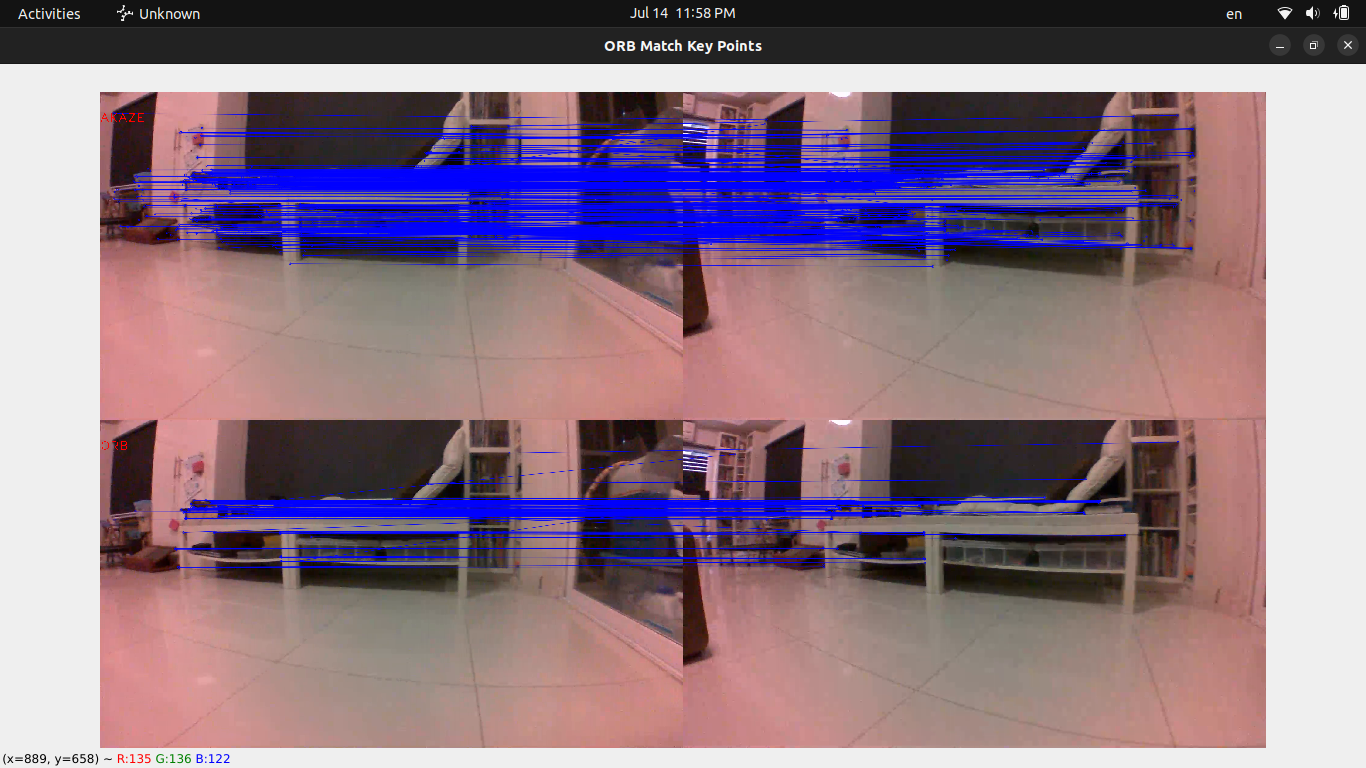
\includegraphics[scale=0.25]{img/matching1.png}
	\end{figure}

    \begin{figure}
		\caption{Q4:  Ratio Test}
		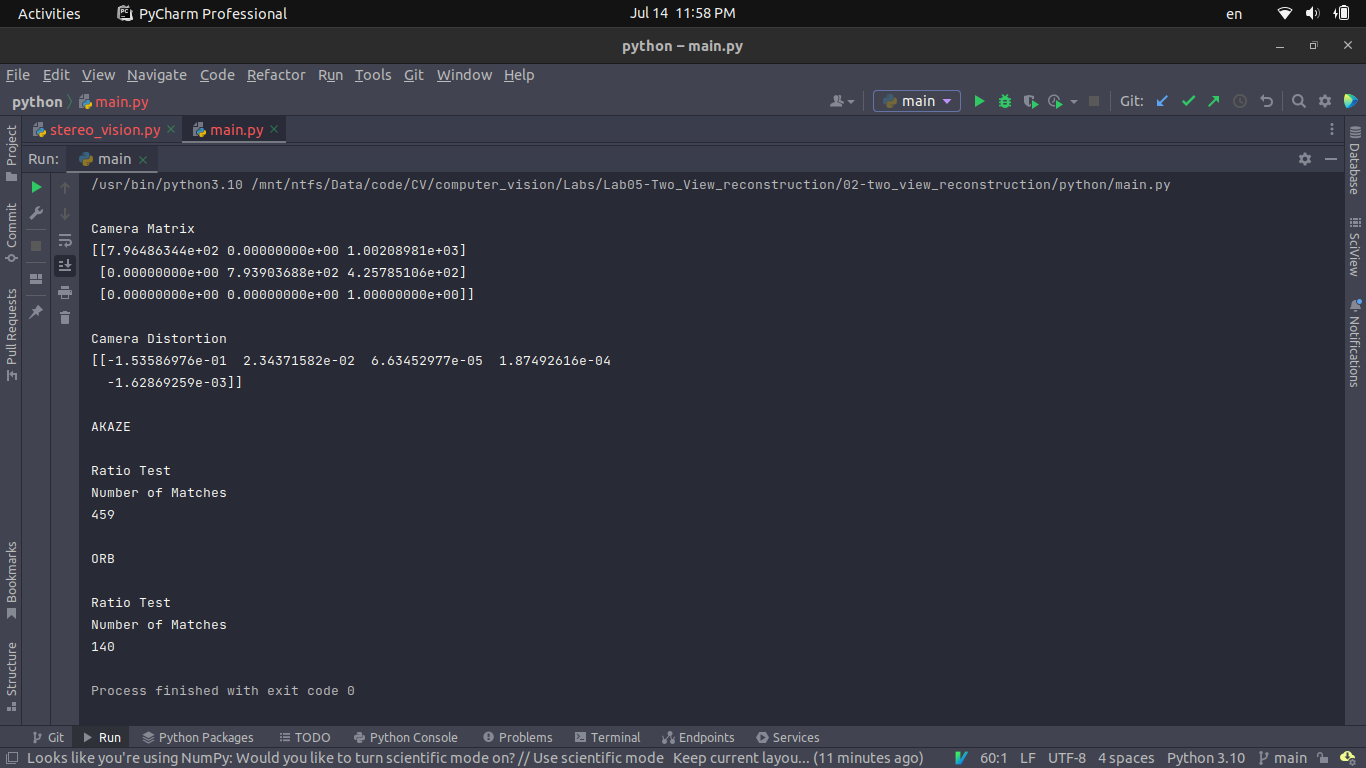
\includegraphics[scale=0.25]{img/matching2.png}
	\end{figure}

    \begin{lstlisting}
# ----------- Match Key Points -----------
nn_match_ratio: float = 0.8
print("\nAKAZE")
akaze_matched_img, akaze_pts1, akaze_pts2, akaze_good_matches = stereo_vision1.match_key_points(nn_match_ratio)
print("\nORB")
orb_matched_img, orb_pts1, orb_pts2, orb_good_matches = stereo_vision2.match_key_points(nn_match_ratio)
cv.putText(akaze_matched_img, "AKAZE", (0, 100), cv.FONT_HERSHEY_PLAIN, 3, (0, 0, 255), 2)
cv.putText(orb_matched_img, "ORB", (0, 100), cv.FONT_HERSHEY_PLAIN, 3, (0, 0, 255), 2)
img = cv.vconcat([akaze_matched_img, orb_matched_img])
show_result_img("ORB Match Key Points", img)

def match_key_points(self, match_ratio=0.8):
    matcher = cv.DescriptorMatcher_create("BruteForce-Hamming")

    matches = matcher.knnMatch(self._img1_desc, self._img2_desc, k=2)

    good_matches = list()
    for i, (m, n) in enumerate(matches):
        if m.distance < match_ratio * n.distance:
            good_matches.append(m)
    pts1 = np.array([self._img1_kps[m.queryIdx].pt for m in good_matches], dtype=np.float32)
    pts2 = np.array([self._img2_kps[m.trainIdx].pt for m in good_matches], dtype=np.float32)

    print("\nRatio Test")
    print("Number of Matches")
    print(pts1.shape[0])

    res_img = cv.drawMatches(self.img1, self._img1_kps, self.img2, self._img2_kps, good_matches, None, (255, 0, 0),
                            (255, 0, 0), flags=2)

    self._pts1 = pts1
    self._pts2 = pts2
    self._good_matches = good_matches
    return res_img, pts1, pts2, good_matches
    \end{lstlisting}

    \section{Q5: Essential Matrix}
    Find essential matrix and use it to get better correspondences.

    \begin{figure}
		\caption{Q5: Matching Using Essential Matrix}
		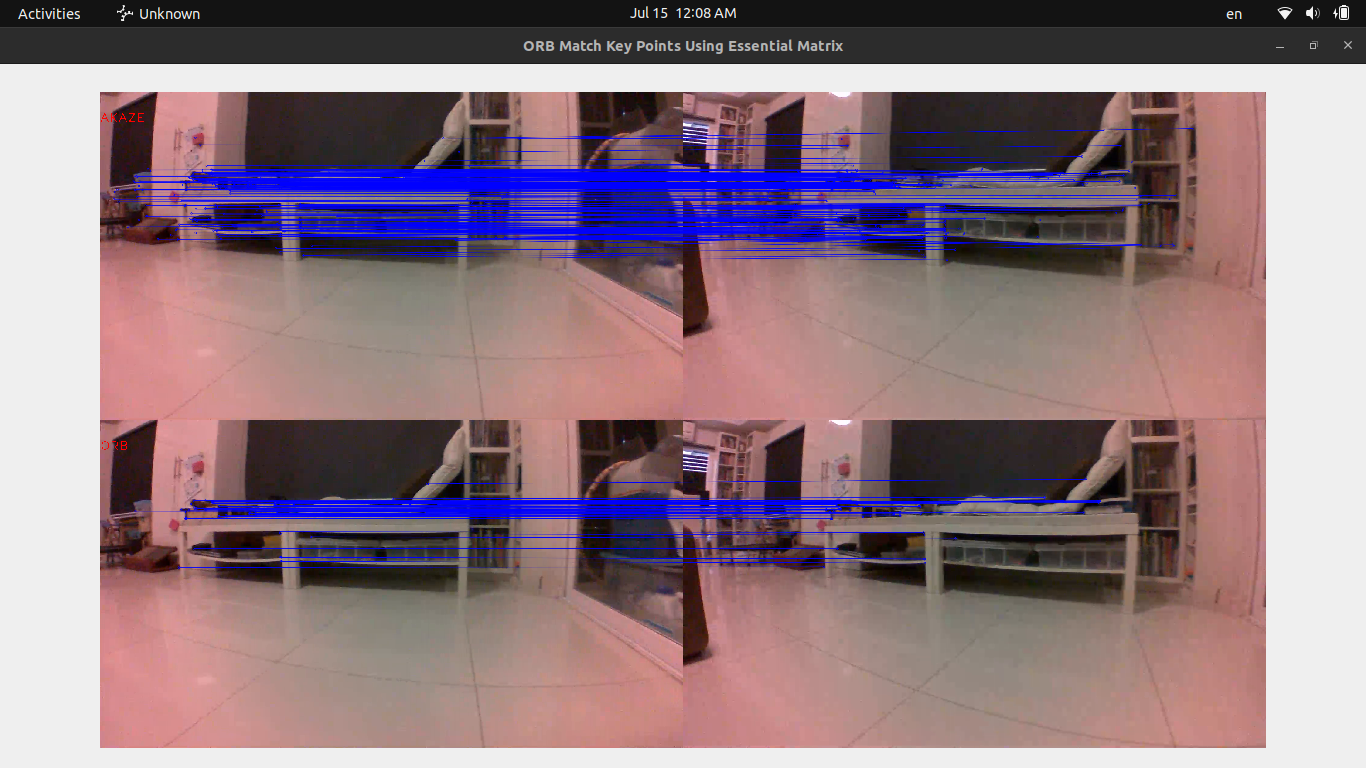
\includegraphics[scale=0.25]{img/essential_matrix.png}
	\end{figure}
    
    \begin{figure}
		\caption{Q5: Essential Matrix Output}
		
\includegraphics[scale=0.25]{img/essential_matrix2.png}
	\end{figure}

    \begin{lstlisting}
  # ----------- Find Essential Matrix -----------
akaze_essential_img, akaze_essential_matrix, akaze_essential_pts1, akaze_essential_pts2, akaze_new_good_matches = \
    stereo_vision1.find_essential_matrix(akaze_pts1, akaze_pts2)
orb_essential_img, orb_essential_matrix, orb_essential_pts1, orb_essential_pts2, orb_new_good_matches = \
    stereo_vision2.find_essential_matrix(orb_pts1, orb_pts2)

cv.putText(akaze_essential_img, "AKAZE", (0, 100), cv.FONT_HERSHEY_PLAIN, 3, (0, 0, 255), 2)
cv.putText(orb_essential_img, "ORB", (0, 100), cv.FONT_HERSHEY_PLAIN, 3, (0, 0, 255), 2)
img = cv.vconcat([akaze_essential_img, orb_essential_img])
show_result_img("ORB Match Key Points Using Essential Matrix", img)

def find_essential_matrix(self, points1, points2):
    essential_matrix, mask = cv.findEssentialMat(points1, points2, self.camera_mtx, cv.FM_RANSAC)
    print("\nEssential Matrix")
    print(essential_matrix)
    pts1 = points1[mask.ravel() == 1]
    pts2 = points2[mask.ravel() == 1]
    new_good_matches = [match for match, m in zip(self._good_matches, mask.ravel() == 1) if m]

    print("\nUsing Essential Matrix")
    print("Number of Matches")
    print(len(new_good_matches))

    res_img = cv.drawMatches(self.img1, self._img1_kps, self.img2, self._img2_kps, new_good_matches, None,
                            (255, 0, 0), (255, 0, 0), flags=2)

    self.essential_matrix = essential_matrix
    self._essential_pts1 = pts1
    self._essential_pts2 = pts2
    self._essential_matches = new_good_matches

    return res_img, essential_matrix, pts1, pts2, new_good_matches
    \end{lstlisting}

    Verify essential matrix
    \begin{lstlisting}
# ----------- Verify Essential Matrix -----------
print("\nVerify essential matrix for AKAZE")
akaze_result = stereo_vision1.verify_essential_matrix(akaze_essential_pts1, akaze_essential_pts2, akaze_essential_matrix)
print(akaze_result)
print("\nVerify essential matrix for ORB")
orb_result = stereo_vision1.verify_essential_matrix(orb_essential_pts1, orb_essential_pts2, orb_essential_matrix)
print(orb_result)

def verify_essential_matrix(self, points1, points2, essential_matrix):
    x = np.concatenate((points1, np.ones((points1.shape[0], 1))), axis=1).T
    x_prime = np.concatenate((points2, np.ones((points2.shape[0], 1))), axis=1).T
    k = self.camera_mtx
    k_inv = np.linalg.inv(k)
    e = essential_matrix
    result = x.T @ k_inv.T @ e @ k_inv @ x_prime
    result = result.astype(np.int32)
    return result
    \end{lstlisting}

    \begin{figure}
		\caption{Q5: Verifying Essential Matrix}
		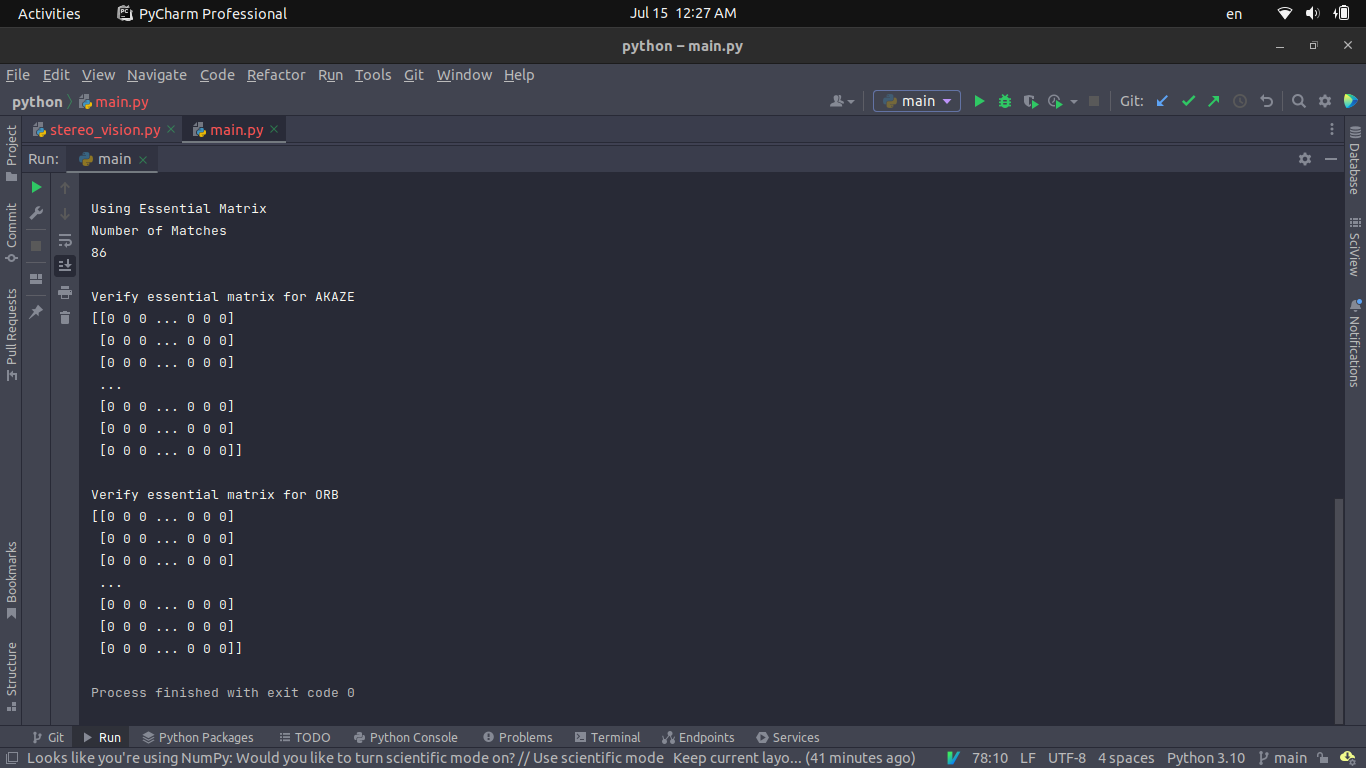
\includegraphics[scale=0.25]{img/essential_matrix3.png}
	\end{figure}
    
    \section{Q6: Undistored Matching}

    \begin{figure}
		\caption{Q6: Undistored Matching}
		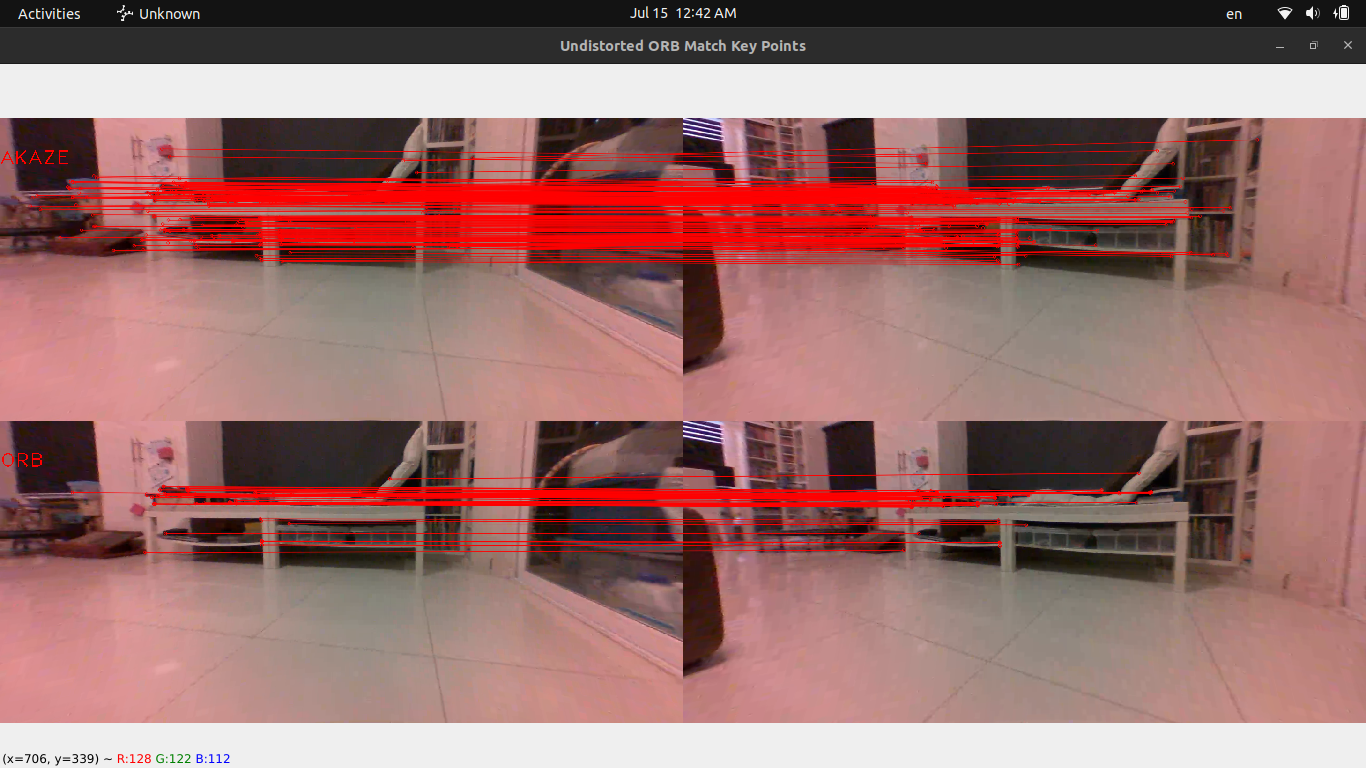
\includegraphics[scale=0.25]{img/undistorted_matching.png}
	\end{figure}

    \begin{lstlisting}
# ----------- Undistorted Matches -----------
akaze_undistorted_matches = stereo_vision1.undistorted_matches(left_img, right_img, akaze_img1_kps, akaze_img2_kps, akaze_new_good_matches)
orb_undistorted_matches = stereo_vision2.undistorted_matches(left_img, right_img, orb_img1_kps, orb_img2_kps, orb_new_good_matches)

cv.putText(akaze_undistorted_matches, "AKAZE", (0, 100), cv.FONT_HERSHEY_PLAIN, 3, (0, 0, 255), 2)
cv.putText(orb_undistorted_matches, "ORB", (0, 100), cv.FONT_HERSHEY_PLAIN, 3, (0, 0, 255), 2)
img = cv.vconcat([akaze_undistorted_matches, orb_undistorted_matches])
show_result_img("Undistorted ORB Match Key Points", img)

def undistorted_matches(self, image1, image2, image1_kps, image2_kps, good_matches):
    undistorted_img1, img1_new_cam_mtx, img1_x, img1_y = self._undistorted_image(image1)
    img1_new_kps = self._undistorted_key_points(image1_kps, img1_new_cam_mtx, img1_x, img1_y)

    undistorted_img2, img2_new_cam_mtx, img2_x, img2_y = self._undistorted_image(image2)
    img2_new_kps = self._undistorted_key_points(image2_kps, img2_new_cam_mtx, img2_x, img2_y)

    res_img = cv.drawMatches(undistorted_img1, img1_new_kps, undistorted_img2, img2_new_kps, good_matches, None,
                                (0, 0, 255), (0, 0, 255), flags=2)
    return res_img
    \end{lstlisting}

    \section{Q7: Epipolar Lines}
    
    \begin{figure}
		\caption{Q7: Epipolar Lines}
		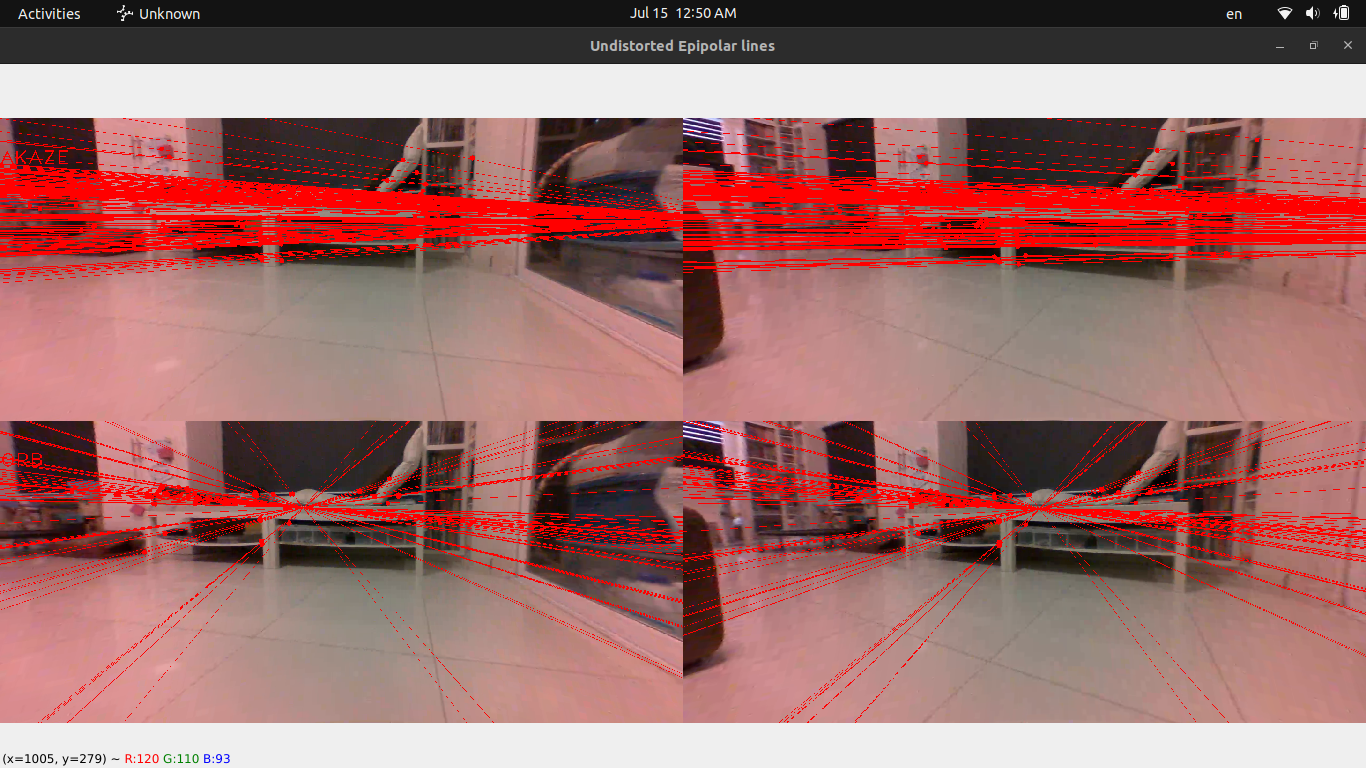
\includegraphics[scale=0.25]{img/epipolar_lines.png}
	\end{figure}

    \begin{lstlisting}
def find_fundamental_matrix(self, essential_matrix):
    mat_k = self.camera_mtx
    mat_k_inv = np.linalg.inv(mat_k)
    mat_k_prime = self.camera_mtx
    mat_k_prime_inv = np.linalg.inv(mat_k_prime)

    fundamental_matrix = mat_k_inv.T @ essential_matrix @ mat_k_prime_inv
    print("\nFundamental Matrix")
    print(fundamental_matrix)

    self.fundamental_matrix = fundamental_matrix

    return fundamental_matrix

@staticmethod
def _draw_lines(image1, image2, lines, points1, points2, color):
    r, c = image1.shape[:2]
    for r, pt1, pt2 in zip(lines, points1, points2):
        x0, y0 = map(int, [0, -r[2] / r[1]])
        x1, y1 = map(int, [c, -(r[2] + r[0] * c) / r[1]])
        image1 = cv.line(image1, (x0, y0), (x1, y1), color, 1)
        image1 = cv.circle(image1, tuple(pt1), 5, color, -1)
        image2 = cv.circle(image2, tuple(pt2), 5, color, -1)
    return image1, image2

def find_epipolar_lines(self, image1, image2, points1, points2, fundamental_matrix, color):
    img1 = image1.copy()
    img2 = image2.copy()
    r_epi_lines = cv.computeCorrespondEpilines(points2.reshape(-1, 1, 2), 2, fundamental_matrix)
    r_epi_lines = r_epi_lines.reshape(-1, 3)

    l_epi_lines = cv.computeCorrespondEpilines(points1.reshape(-1, 1, 2), 1, fundamental_matrix)
    l_epi_lines = l_epi_lines.reshape(-1, 3)

    pts1 = points1.astype(np.int32)
    pts2 = points2.astype(np.int32)

    image5, image6 = self._draw_lines(img1, img2, r_epi_lines, pts1, pts2, color)
    image7, image8 = self._draw_lines(img2, img1, l_epi_lines, pts2, pts1, color)
    res_img = cv.hconcat([image5, image7])

    return res_img, l_epi_lines, r_epi_lines

def undistorted_epipolar_lines(self, image1, image2, image1_pts, image2_pts):
    undistorted_img1, img1_new_cam_mtx, img1_x, img1_y = self._undistorted_image(image1)
    undistorted_img2, img2_new_cam_mtx, img2_x, img2_y = self._undistorted_image(image2)

    undistorted_pts1 = self._undistorted_points(image1_pts, img1_new_cam_mtx, img1_x, img1_y)
    undistorted_pts2 = self._undistorted_points(image2_pts, img2_new_cam_mtx, img2_x, img2_y)

    _, essential_matrix, essential_pts1, essential_pts2, _ = self.find_essential_matrix(undistorted_pts1,
                                                                                        undistorted_pts2)
    fundamental_matrix = self.find_fundamental_matrix(essential_matrix)

    res_img, _, _ = self.find_epipolar_lines(undistorted_img1, undistorted_img2, undistorted_pts1, undistorted_pts2,
                                                fundamental_matrix, (0, 0, 255))
    return res_img
    \end{lstlisting}    

    \section{Q8:  Factorization of Essential Matrix}

    \begin{figure}
		\caption{Q8: Factorization of Essential Matrix}
		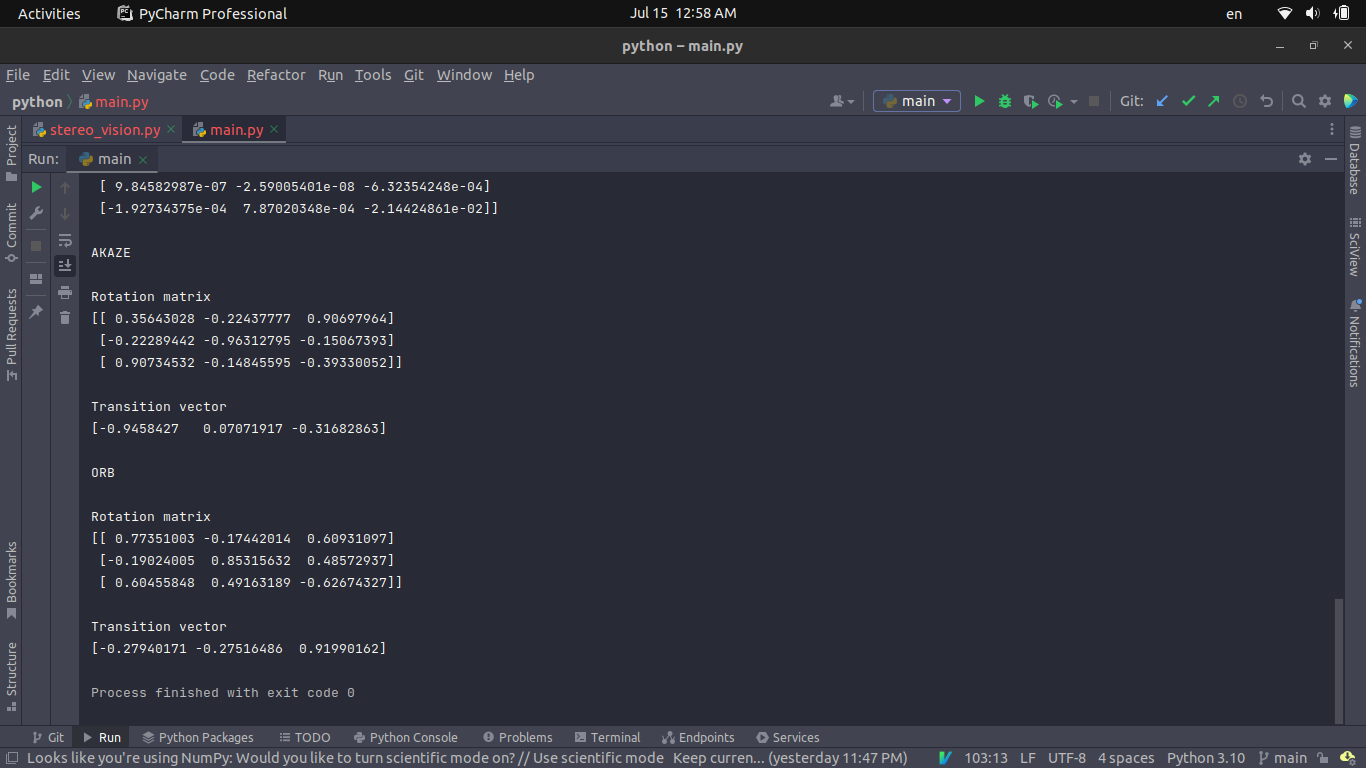
\includegraphics[scale=0.25]{img/factorization.png}
	\end{figure}

    \begin{lstlisting}
# ----------- Decompose essential matrix -----------
print("\nAKAZE")
akaze_rotation, akaze_transition = stereo_vision1.decompose_essential_matrix()
print("\nORB")
orb_rotation, orb_transition = stereo_vision2.decompose_essential_matrix()

def decompose_essential_matrix(self):
    mat_u, mat_s, mat_vt = np.linalg.svd(self.essential_matrix)
    mat_w = np.array([
        [0.0, -1.0, 0.0],
        [1.0, 0.0, 0.0],
        [0.0, 0.0, 1.0]
    ])
    mat_r = mat_u @ mat_w @ mat_vt
    mat_t = mat_u[:, 2]

    print("\nRotation matrix")
    print(mat_r)
    print("\nTransition vector")
    print(mat_t)

    self.rotation_mtx = mat_r
    self.transition_vec = mat_t

    return mat_r, mat_t
    \end{lstlisting}

    \section{Q9:  Recover Relative Pose}
    
    \begin{figure}
		\caption{Q9: AKAZE Points Cloud}
		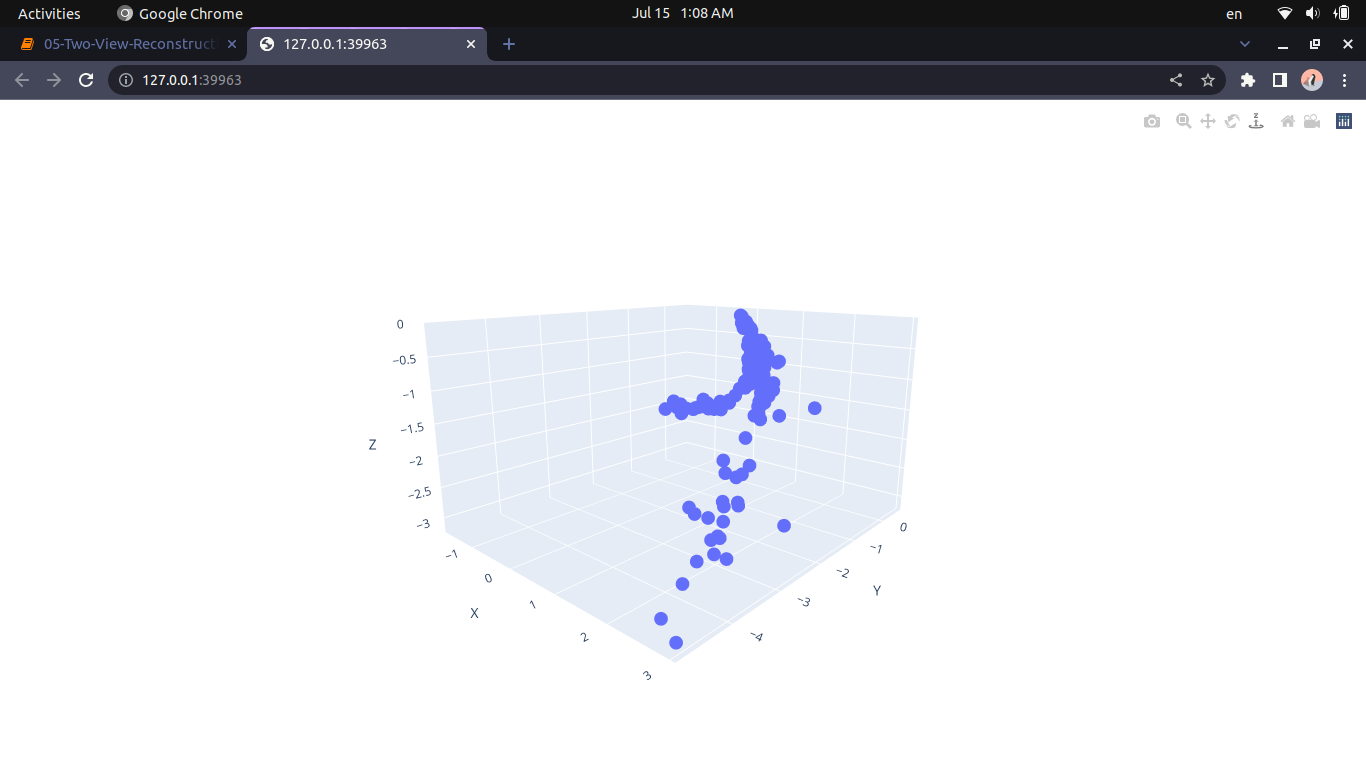
\includegraphics[scale=0.25]{img/akaze_cloud_points.png}
	\end{figure}

    \begin{figure}
		\caption{Q9: ORB Points Cloud}
		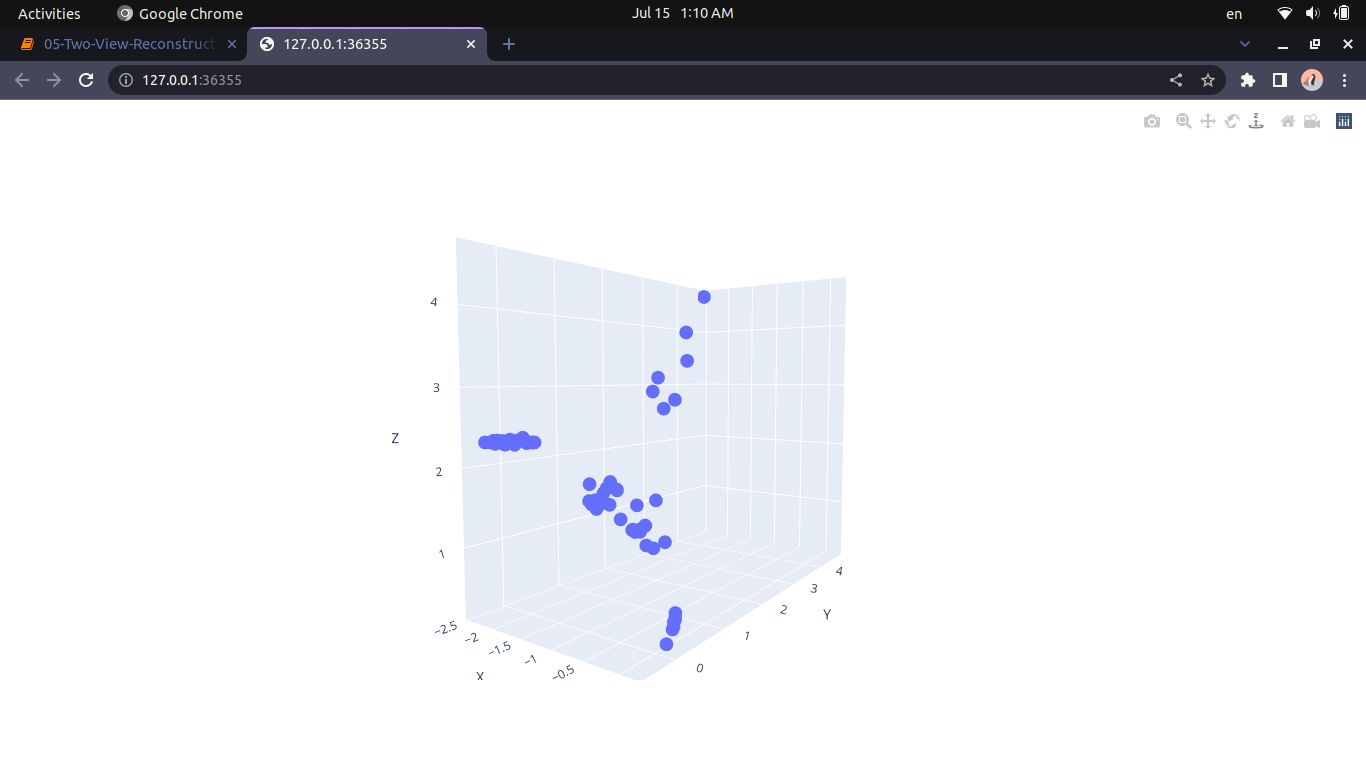
\includegraphics[scale=0.25]{img/orb_cloud_points.png}
	\end{figure}

    \begin{lstlisting}
import pandas as pd
import plotly.express as px
# ----------- Recover Relative Poses -----------
akaze_fundamental_matrix = stereo_vision1.find_fundamental_matrix(akaze_essential_matrix)
akaze_points_3d = stereo_vision1.recover_relative_pose(akaze_essential_pts1,  akaze_essential_pts2, akaze_fundamental_matrix,
                                                    akaze_essential_matrix)

df = pd.DataFrame(akaze_points_3d, columns=["X", "Y", "Z"])
fig = px.scatter_3d(df, x="X", y="Y", z="Z")
fig.show()

orb_fundamental_matrix = stereo_vision2.find_fundamental_matrix(orb_essential_matrix)
orb_points_3d = stereo_vision2.recover_relative_pose(orb_essential_pts1,  orb_essential_pts2, orb_fundamental_matrix,
                                                        orb_essential_matrix)

df = pd.DataFrame(orb_points_3d, columns=["X", "Y", "Z"])
fig = px.scatter_3d(df, x="X", y="Y", z="Z")
fig.show()

def recover_relative_pose(self, points1, points2, fundamental_matrix, essential_matrix):
    pts1 = points1.reshape(1, -1, 2)
    pts2 = points2.reshape(1, -1, 2)

    pts1, pts2 = cv.correctMatches(fundamental_matrix, pts1, pts2)

    _, rotation, translation, mask = cv.recoverPose(essential_matrix, pts1, pts2, self.camera_mtx)
    print("\nRotation: ")
    print(rotation)
    print("\nTranslation: ")
    print(translation)

    projection1 = self.camera_mtx @ np.concatenate((rotation, translation), axis=1)
    projection2 = self.camera_mtx @ np.concatenate((np.eye(3), np.zeros((3, 1))), axis=1)
    print("\nProjection 1: ")
    print(projection1)
    print("\nProjection 2: ")
    print(projection2)

    pts1 = pts1.reshape(2, -1)
    pts2 = pts2.reshape(2, -1)

    points_4d = cv.triangulatePoints(projection1, projection2, pts1, pts2)
    points_4d = points_4d / np.tile(points_4d[-1, :], (4, 1))
    points_3d = points_4d[:3, :].T
    return points_3d
    \end{lstlisting}
\end{document}